\documentclass[11pt,letterpaper,twocolumn]{article}

\usepackage{mathpazo,fancyhdr,graphicx,wrapfig,color,sidecap,colortbl,bm,cite,sidecap}
\usepackage{xcolor}
\usepackage{listings}

\lstdefinestyle{yaml}{
     basicstyle=\color{blue}\footnotesize,
     rulecolor=\color{black},
     string=[s]{'}{'},
     stringstyle=\color{blue},
     comment=[l]{:},
     commentstyle=\color{black},
     morecomment=[l]{-}
 }


\usepackage[labelfont=bf,small]{caption}
\usepackage{booktabs}
 
\usepackage{subcaption}
 \usepackage[english]{babel}
 
 \usepackage{algorithm}
\usepackage{algpseudocode}
 
\definecolor{Red}{rgb}{0.6,0.1,0.2}

 \usepackage{tikz}
\newcommand*\circled[1]{\tikz[baseline=(char.base)]{
            \node[shape=circle,draw,inner sep=1.5pt] (char) {#1};}}
            
            
\renewcommand{\refname}{References cited}

\setlength{\belowcaptionskip}{-5pt}

\textwidth=6.5in \textheight 9in \oddsidemargin=0in \topmargin=-0.5in

\sloppy

\pagestyle{fancy} 
\lhead{}
\chead{}
\rhead{\fontsize{9.4}{13} \sc Cover Page} 
\lfoot{\small \sc }  %\lfoot{\small \sc d. Project Description}
\cfoot{}
\rfoot{}
\renewcommand{\headrulewidth}{1pt}
\renewcommand{\footrulewidth}{1pt}

%\renewcommand\thesection{\textsc{d.}\,\arabic{section}}



\usepackage{verbatim}
\usepackage{enumitem}
\usepackage{multirow}
\usepackage{amsmath,amsfonts}
\newcommand{\thickhline}{\noalign{\hrule height 1.0pt}}
%\usepackage[letter]{aspdac2e}
\usepackage{multirow,multicol}

\newcommand{\ten}[1]{\mathbfcal{#1}}   %mathcal
\newcommand{\mat}[1]{\mathbf{#1}}


\DeclareMathAlphabet\mathbfcal{OMS}{cmsy}{b}{n}


\newcommand{\zhang}[1]{\textcolor{blue}{#1}}

\title{
\begin{medium}
\vspace{15pt}
  \textsf{Nimble - The Marketplace of Intents}
\end{medium} 

\begin{small}
\vspace{15pt}
  \textsf{\emph{A Permissionless and Extensible Protocol for an Intent Economy}}\\
  % \textsf{v1.0}
\vspace{-20pt}
\end{small} 
\date{October 10, 2023}
% \date{\today}
}

\setcounter{page}{1}

\thispagestyle{fancy}
\lhead{}
\chead{}
\rhead{\small \sc Nimble - The Marketplace of Intents}
\lfoot{\small \sc $\copyright$2023 Nimble Technology. All rights reserved.}
\rfoot{\thepage}
\renewcommand{\headrulewidth}{1pt}
\renewcommand{\footrulewidth}{1pt}


\begin{document}
\maketitle

\begin{abstract}
Today’s blockchain systems are obscure. Users of dApps must perform low-level operations to complete basic tasks. Developers seeking to launch a new dApp must learn a new technical stack. Such system complexity is preventing mainstream adoption of Web3 technologies by users and developers alike.

This paper presents Nimble, the \emph{ecosystem's first} marketplace of intents. Nimble solves this notorious problem while improving Web3 composability and decentralization. User interactions with dApps (e.g. GUI clicks and natural language queries) are modeled using intents. Intents are mapped to a standard DSL using LLMs and other intent understanding techniques. Dispatchers route intent DSL to specialized solvers, which execute the instructions on-chain. Solvers compete for intents, minimizing harmful MEV. The protocol is open, decentralized, and extensible.
\end{abstract}

\section{Introduction}
\label{sec:introduction}
% Problem
Today's blockchain user experience is comparable to the early days of computing.
Computer users had to understand hardware configurations, install drivers, and
interact with applications through command lines or minimal user interfaces.
Modern Web3 users face similar technical overhead. Low-level operations like transactions, swaps, and bridging are part of the basic vocabulary of Web3 users. Developers cannot build platform-agnostic applications, which forces users to understand the differences between blockchains, possess multiple wallets, and manually track their assets. 

\begin{figure}[t]
\centering
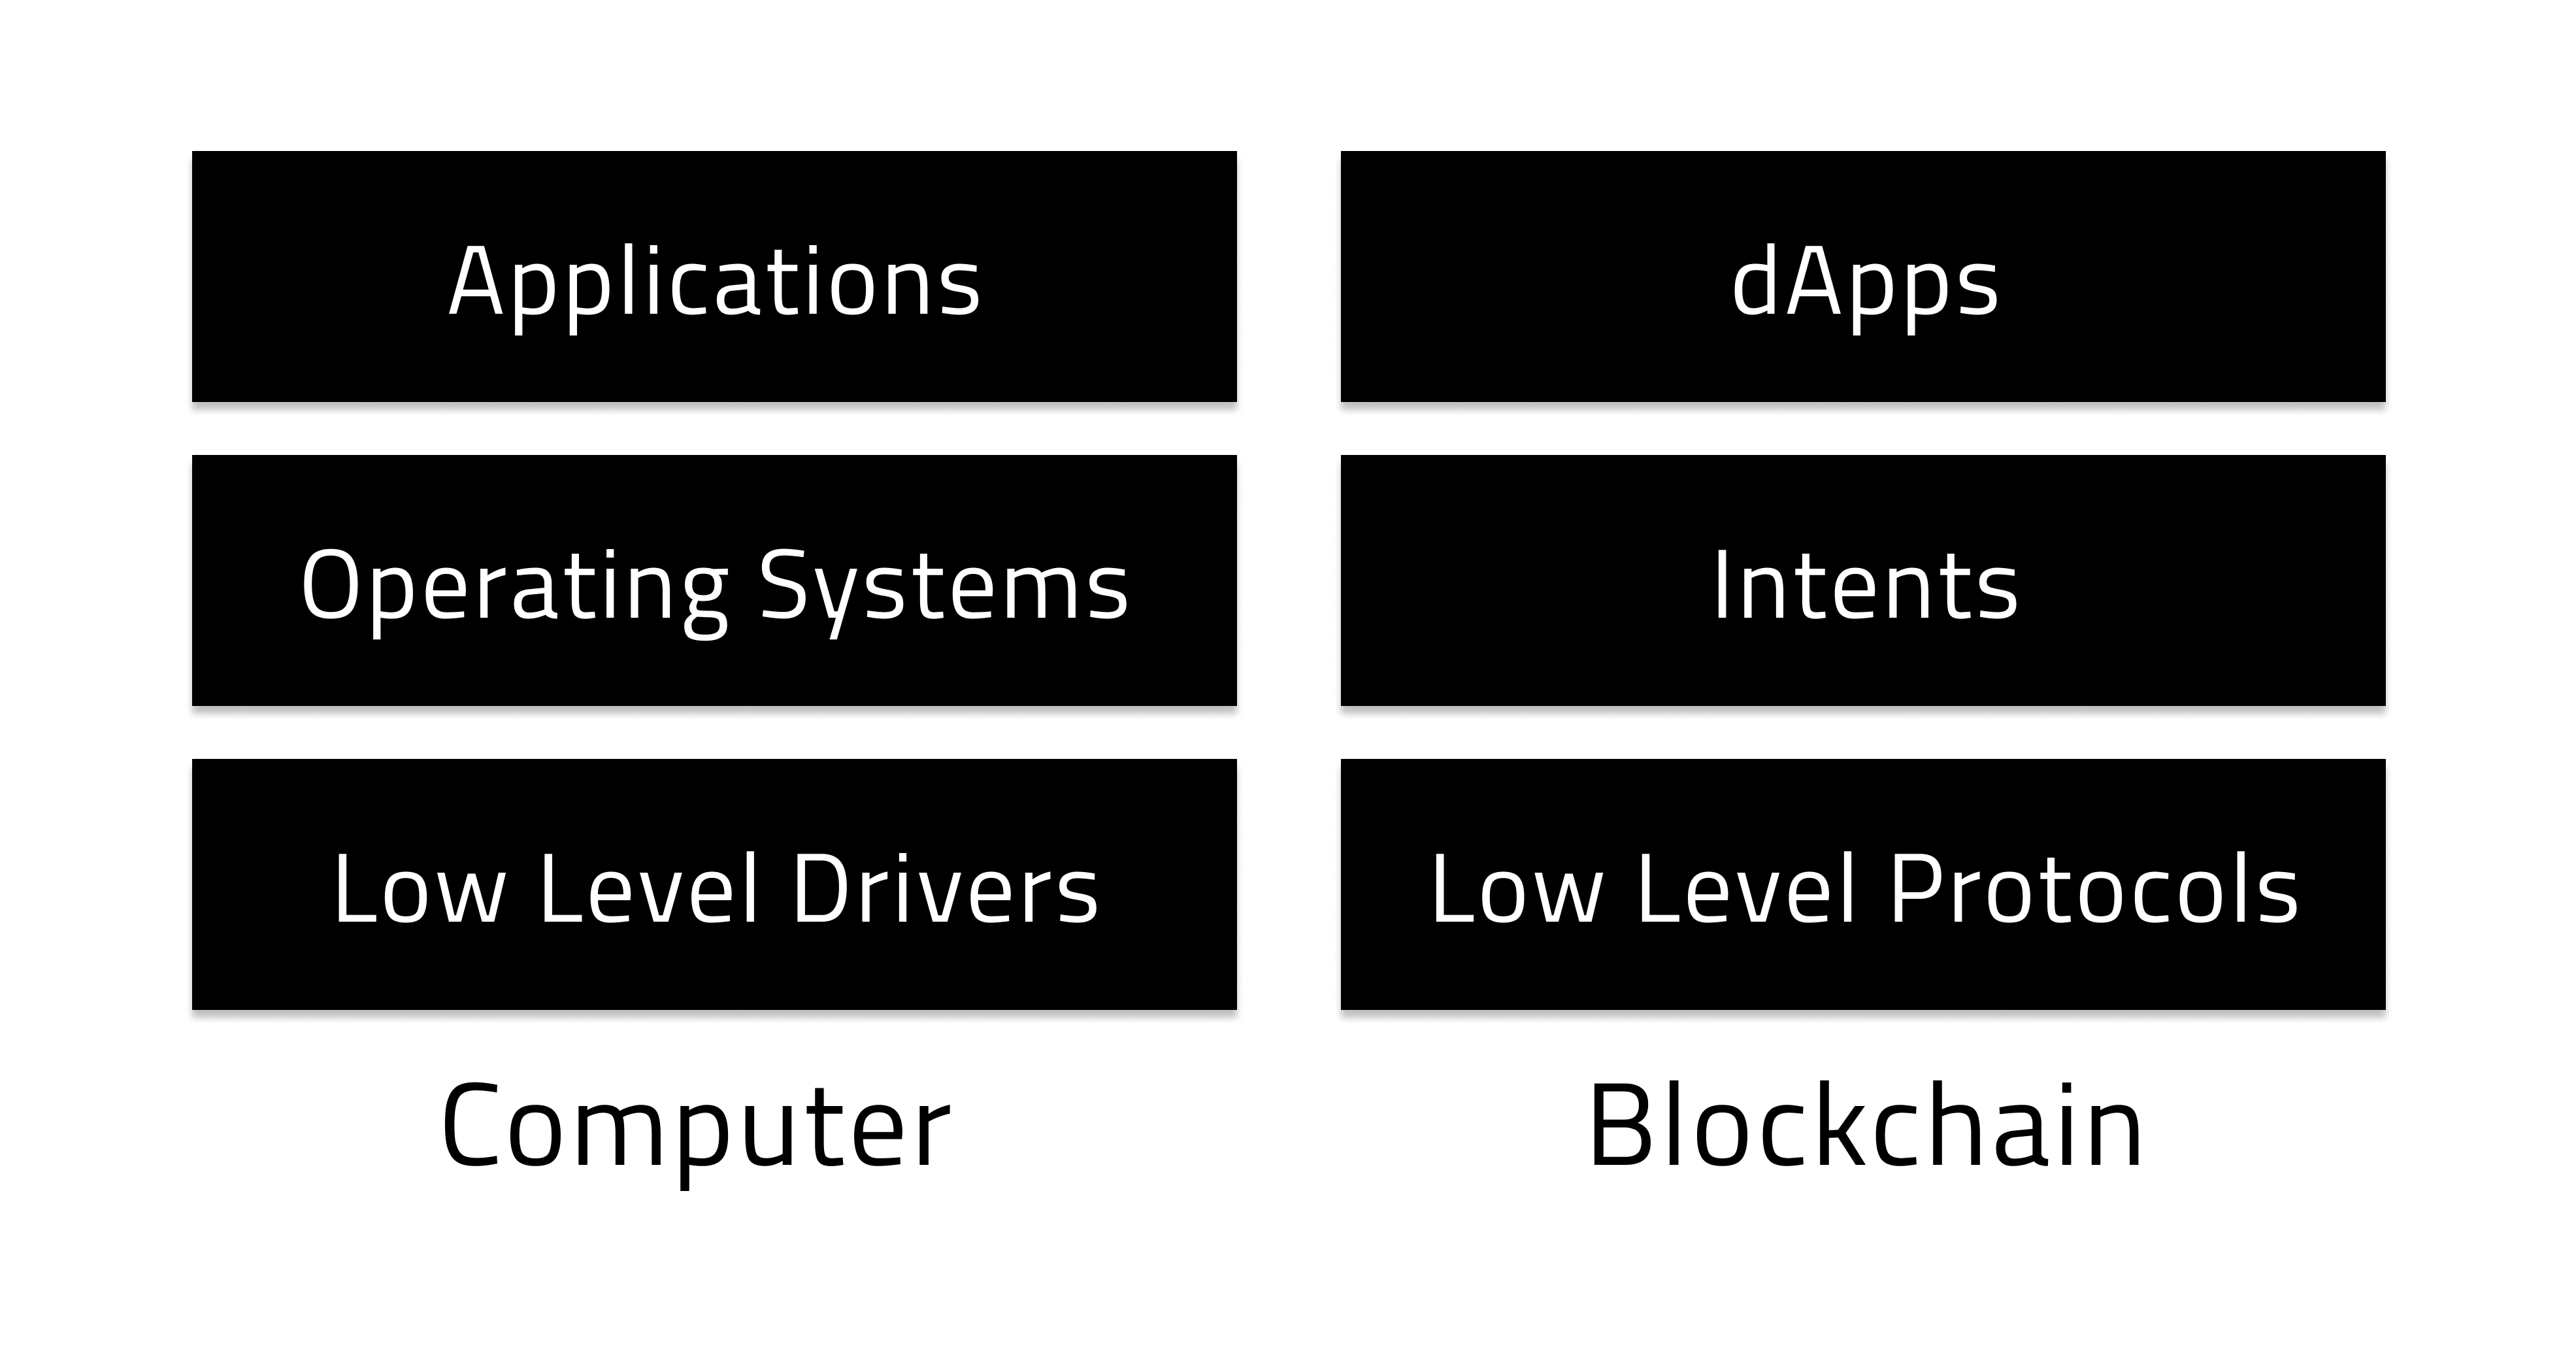
\includegraphics[width=3in]{fig/operating-system-analogy-hr.png}
\caption{Nimble abstracts low-level blockchain operations away from developers, serving as an operating system for Web3. It is an
abstraction layer on top of L1s $\&$ L2s.} 
\label{fig:os-analogy}
\vspace{0pt}
\end{figure}

% Vision
Nimble’s vision is to enable a marketplace of intents.
As a Web3 portal protocol, Nimble sits on top of blockchains, L2s, and bridges. It hides the underlying complexity of blockchain systems, providing a unified interface for all compatible Web3 systems. Developers interact with Nimble directly without the need to understand fundamental operations. Such developers can easily build cross-platform dApps, and low-level operations can be completely hidden from end users.

Our development philosophy is governed by principles of \emph{decentralization}, \emph{openness}, and \emph{inclusion}. Decentralization is achieved with an overlay network governing the messaging, payload parsing, and
intent processing. The protocol is open to use with publicly published SDKs and APIs. Community members can contribute to the code development and product direction discussions by participating in the DAO.

% discuss all the physical network functionalties before the real market discussions
% network operators
The Nimble network is a set of validators forming an overlay network, 
running intent processing and reaching consensus for intent operations. A validator is a set of one or more network operators.
Each operator is a physical machine running one or more conceptual modules.
It is connected with multiple others on the network for resilience against
operator departures. New operators join the network by building connections with existing
network operators.
% intent pools
Intent pools consist of two key operations functioning in a decentralized manner:
intent propagation and discovery.
The overlay network adopts gossip protocols for intent propagation
and distributed hash tables for intent discovery \cite{kaashoek2003koorde, jin2011network}. Each intent request arrives at one or more operators.
Each operator has a partial view of the network intent pool, called intent maps.
Intent maps are propagated across the network to get a holistic view of intents among operators. Intent discovery requests are processed in a similar manner.
% consensus
Using a Proof of Stake algorithm, validators reach consensus on intent operations, such as intent interpretation and dispatching, instead of transactions themselves.

% real market modules
Nimble marketplace consists of the following three decentralized markets:
\begin{itemize}
\item \textbf{The Interpretation Market.} The intent recognizer accepts general format intents
and translates them into concrete intent operations. Intents are represented as an intent
taxonomy forest for ontology. Each intent category (e.g., trade and token) is an independent tree defined by a standard DSL. Specific intent operations are leaves on the trees. LLMs and rule engines are adopted for natural language intent understanding (i.e., map user intents into tree leaves).

\item \textbf{The Dispatching Market.} Structured intents from the interpretation market formulate the intent pool. Intent dispatchers monitor such an intent pool and route intents
to the right auctions. Dispatchers exchange intent maps to expand the visibility of the intent pool. With intent operations specified by the DSL, dispatchers can accurately and efficiently discover the specific auctions. This match-making is analogous to matching riders and drivers by ride-hailing apps.

\item \textbf{The Settlement Market.} The settlement market runs a unified auction layer with
a modular, composable, and multi-stage design for scalability. In an ideal world, optimizing
intent execution is a centralized mechanism design problem. However, the growth of
intent categories introduces the notorious dimensionality problem, making the optimization
computationally prohibitive. While network traffic remains low, it may be possible to maintain a central auction for solvers. As network volume grows, it will become necessary to run modular auctions. 

In modular auctions, solvers will compete in each child auction for the portion of the user’s intent they can fulfill. Generic solvers may fulfill the entirety of a user’s intent, while specialized solvers may fulfill only a single operation in a highly optimized way. Modular auctions are created to satisfy atomic intent operations, and composite auctions are created to satisfy operation sets. Through composability and modularity, the protocol can generate optimal solutions from solvers without sacrificing performance.

In the final stage of the auction, solutions from solvers are submitted to Bundlers to finalize the bid. These bundlers are a specialized type of solver that combines solutions into a completed bid.

This multi-stage mechanism design is adopted for flexibility, scalability, and extensibility \cite{sandholm2007automated}.

\end{itemize}

% paper structure
Section \ref{sec:background} discusses related work and existing intent solutions.
Section \ref{sec:marketplace} details the marketplace infrastructure design.
Section \ref{sec:mechanism} illustrates the theoretical aspect of the multi-stage mechanism
design. Section \ref{sec:consensus} summarizes the consensus protocol. Conclusions follow this in Section \ref{sec:conclusion}.

\section{Background}
\label{sec:background}
This section discusses the evolution of decentralization technologies, natural language deep learning techniques, and existing intent solutions. 

\subsection{Bitcoin}
In the evolution of blockchain, Bitcoin was the first viable solution \cite{nakamoto2008bitcoin}.
Bitcoin is a decentralized digital currency that can be transferred on the Bitcoin network. The peer-to-peer network of nodes running Bitcoin software maintains the blockchain, which is a public record of bitcoin transactions. The network nodes independently store a copy of the blockchain and validate transactions, appending them to their own copies of the blockchain and transmitting the additions to other nodes. In every epoch, a new block that contains a new batch of valid transaction records is added to the blockchain and issued to all nodes. The miner nodes do the record-keeping of the blockchain by using their processing power. The easy-to-verify but hard-to-solve proof-of-work (PoW) is required in each new block to be accepted by the rest of the network. Merkel Trees are adopted so non-miners can use the block header to verify a new blockchain without checking all past transactions. Once a new block is accepted by the rest of the network, the miner who successfully solved the problem is rewarded with newly created bitcoins and transaction fees.

\subsection{Ethereum}
After Bitcoin, numerous additional blockchains were built. Among them, Ethereum pioneered the smart contract platform \cite{wood2014ethereum}.
Ethereum inherits the Bitcoin ecosystem's consensus, decentralization, and cryptography. While Bitcoin is limited as a simple ledger, the Ethereum blockchain has a built-in Turing-complete programming language that allows anyone to write smart contracts and develop decentralized applications (dApps) on top of it. Ether (ETH) is the native cryptocurrency of the Ethereum blockchain that is paid to the miners as transaction fees. Due to their autonomous nature under their own logic, Ethereum contracts are often called smart contracts. The code in the contracts is written in Ethereum virtual machine (EVM) code, a low-level, stack-based bytecode language. The EVM is the runtime environment of Ethereum that includes a stack, memory, gas balance, program counter, and persistent storage for all accounts. When a transaction calls a contract's function, the EVM translates and executes the contract's code into stack operations. A transaction sender must pay the miner, who is running the EVM and adding the transaction to the blockchain, a certain amount of gas fee in ETH. The gas fee system can reduce the amount of spam transactions.

\subsection{Proof-of-Stake}
Initially proposed by PeerCoin \cite{king2012ppcoin}, the creation of a scalable Web3 smart contract platform has recently become a focus for the community. Proof-of-Stake (PoS) is more scalable and better suited for general-purpose blockchains like Ethereum. Applications like decentralized finance (DeFi), non-fungible tokens (NFTs), minting, and sales all require high transaction volumes and benefit from improved scalability.
In PoS, a blockchain employs a network of validators who stake their own tokens into a pool to get a chance to validate new transactions. If a validator is chosen to update the blockchain, they receive the reward. A majority consensus has to be reached for a block to be accepted and added to the blockchain. Weighted voting can be adopted to improve the robustness of the consensus, where the weight is determined by the node's profile, such as the amount of stake and reputation.

\subsection{LLMs for Intents}

User intent understanding is well studied in Web2 for personalized search, recommendation, and user growth.
The mainstream approach is to adopt large-scale AI models and knowledge graphs
for named entity tagging and similarity search \cite{vaswani2017attention, wang2023gpt, zou2020survey, ArchImpl19, DLRM19, QuoRemTrick19}.
For example, search queries are processed with spelling corrections,
query segmentation into semantic units, and entity tagging for
such units with human-understandable concepts like place names,
companies, industries, etc. Such concepts (i.e., entities)
are mapped into a graph to represent their relationships. This lays the foundation for a structural
understanding of intents. Another popular approach is representing user queries as embeddings (i.e., a
vector of bits). The intents of the queries and items (i.e., products in e-commerce, articles in
search, and posts in recommendations) are measured by cosine similarity among them. That is, queries with similar
intents and items on similar topics are closer in the mapped space.

\subsection{Intents in Web3}

Nimble is the first to focus on building a trustless marketplace infrastructure
for Web3 intent applications. Anoma builds a privacy blockchain with zero knowledge proofs \cite{anoma2023privacychaincoindesknews}. This is a significant departure from
intents. SUAVE by Flashbots focuses on MEV decentralization with a trusted
execution environment (TEE) for privacy via SGX hardware support. However,
a) SGX can be hacked \cite{murdock2020plundervolt}; and
b) SGX hardware is highly specialized and difficult to acquire as the network scales \cite{severinsen2017secure}. Cowswap, 1inch Fusion, and UniswapX provide dApps which focus on trading \cite{cow2023, 1inchfusion2023, uniswapx2023}. Essential is
building an intent contract standard \cite{essential2023standard} emphasizing intent contracts.

\section{The Marketplace Infrastructure}
\label{sec:marketplace}
Nimble's marketplace infrastructure consists of interpretation, dispatching, and settlement markets. These markets are detailed in this section. The intent sync protocol is also briefly discussed prior to detailed market discussions.

\subsection{IntentSync Protocol}
Gossip protocols and overlay networks are well discussed in the literature on which
intents and other network communications are performed \cite{kaashoek2003koorde, ren2010topbt, zhao2005gridmedia, small2006scaling, dabek2005distributed, jin2011network}. Here, the discussion is focused on the \emph{IntentSync} protocol for application in the Nimble protocol. The
protocol consists of an intent map, intent propagation, and intent pool.

An intent map is a list of intents together with unique intent IDs. It is an atomic buffer
map maintained by each validator. Each validator maintains two intent maps: one for the
general purpose intents from users and the other for the structured intents in DSL formats.
Intent maps are exchanged among validators with the intent propagation algorithm. The
algorithm periodically fetches intent maps from its neighbors (i.e., connected validators).
It merges new intent maps with the existing ones. The algorithm also periodically discovers
new validators as neighbors by removing existing ones with low reputation scores,
computed based on network token stakes and the history of mutual interactions.
The intent pool is a distributed hash table formed by the intent maps.

\subsection{The Interpretation Market}
The Intent recognizer serves as the gateway to the Nimble protocol, acting as the interpreter of user intentions. Its primary function is to bridge the gap between the user's natural language expressions and the protocol's machine-readable understanding. Leveraging Natural Language Processing (NLP) techniques for entity recognition, this layer deciphers user input, extracting the essence of their blockchain-related requests together with rule-based approaches. It translates these intents into a structured format, such as a list of user operations, using an intuitive Intent Query-Based DSL \cite{mernik2005and, kosar2008preliminary, fowler2010domain, hudak1997domain, selic2007systematic}. This layer is essential in ensuring that user interactions are comprehensible to the subsequent layers, creating a seamless and user-friendly entry point to the world of Web3.

\begin{figure}[t]
\centering
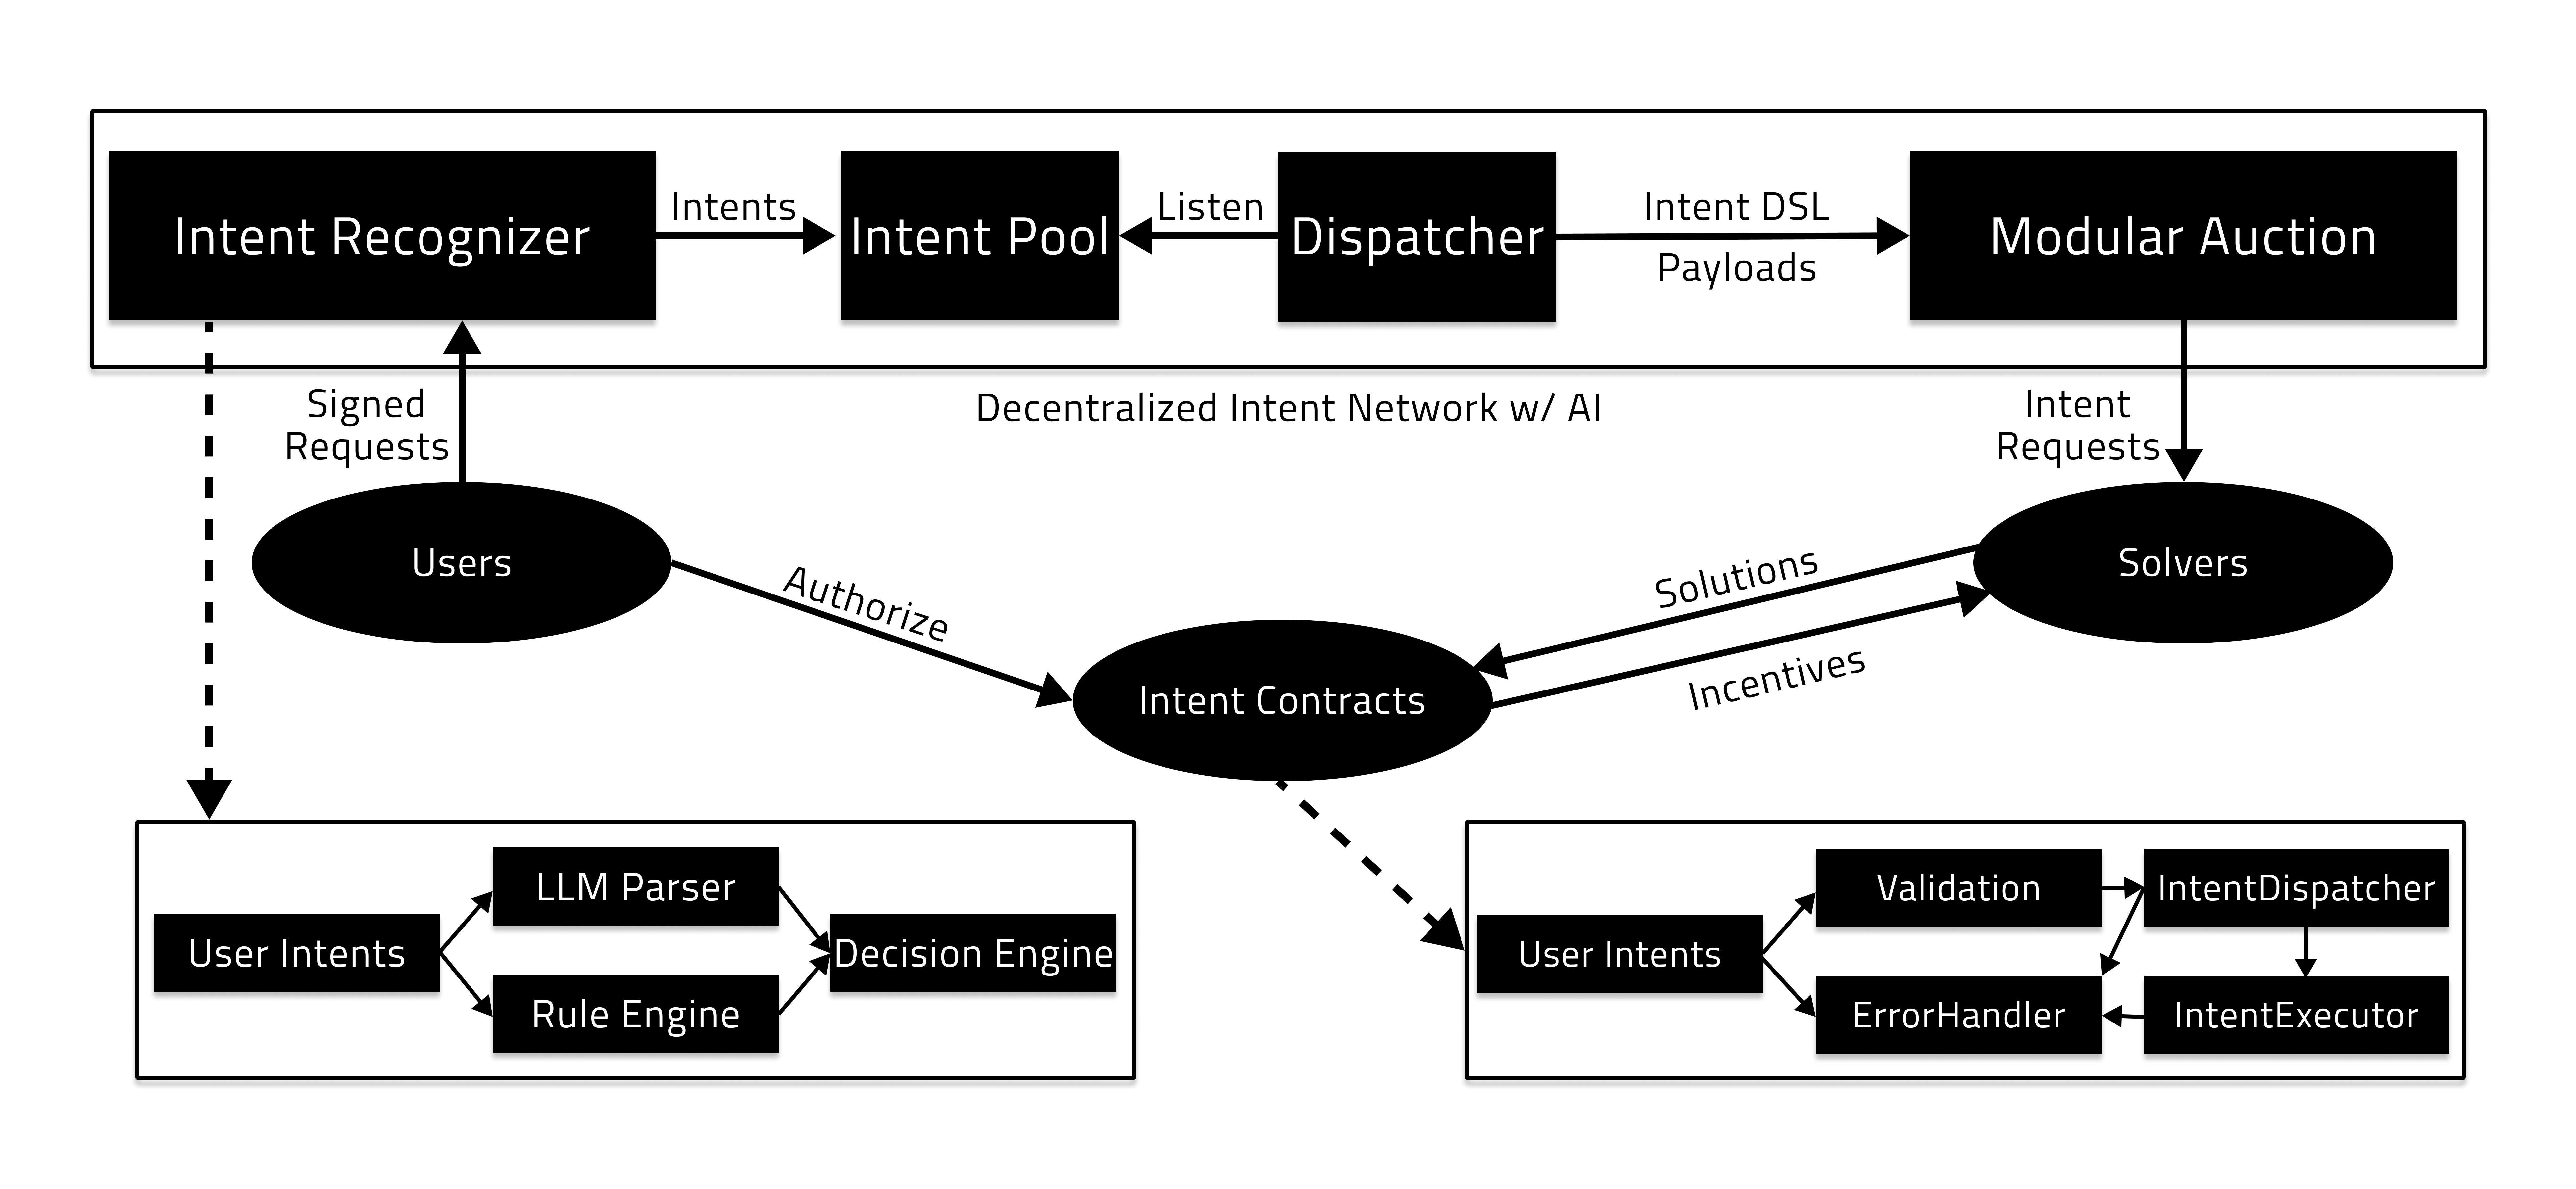
\includegraphics[width=3in]{fig/intent-architecture-hr.png}
\caption{Nimble intent protocol consists of three essential modules that work together seamlessly to facilitate decentralized user interactions with blockchain technologies.
Intent recognizer understands user intents as machine-readable intent operations. Intent operations are published to intent pools. Such pools are a critical component of the intent dispatcher. The intent dispatcher runs a second-price auction for truthful solver bids. Solvers interact with the auction protocol within the dispatcher for intent competitions. Intent contracts provide permissionless on-chain execution.} 
\label{fig:intent-architecture}
\vspace{0pt}
\end{figure}

\begin{itemize}

\item This foundational layer serves as the entry point for user interactions with Web3 components.

\item It utilizes Natural Language Processing (NLP) algorithms and smart contract interfaces to decipher and extract user intent from textual or voice-based inputs.

\item Within the Intent Recognizer, a key component is the utilization of an Intent Query-Based DSL, which bridges users' natural language intents and machine-readable operations.

\item This DSL allows users to express their blockchain-related intentions in a structured and declarative manner, resembling SQL or YAML for ease of use.

\item Users can formulate complex queries or declarative statements that specify the desired blockchain actions, parameters, and conditions.

\item It abstracts the complexities of blockchain interactions into intuitive and human-readable syntax, including smart contract interactions, token transfers, staking, and more.

\item It employs advanced parsing and pattern recognition techniques to translate DSL statements into a list of user operations comprehensible to the protocol.

\end{itemize}
\newline
\newline
\noindent \textbf{Intent Representation.}
Intents are outcome-driven messages signed by users. Intents are desired user-specified states rather than instructions like transactions. They focus on user preferences, the product journey, and the desired protocol outcomes. For extensibility, intents are standardized in both the definitions and understanding. Example intents are:
\begin{itemize}
\item Stake ETH for best yields,
\item Trade USDC for ETH at the optimal price, and
\item Swap USDC for ETH with minimum slippage of $0.1\%$.
\end{itemize}


\begin{figure}[t]
\centering
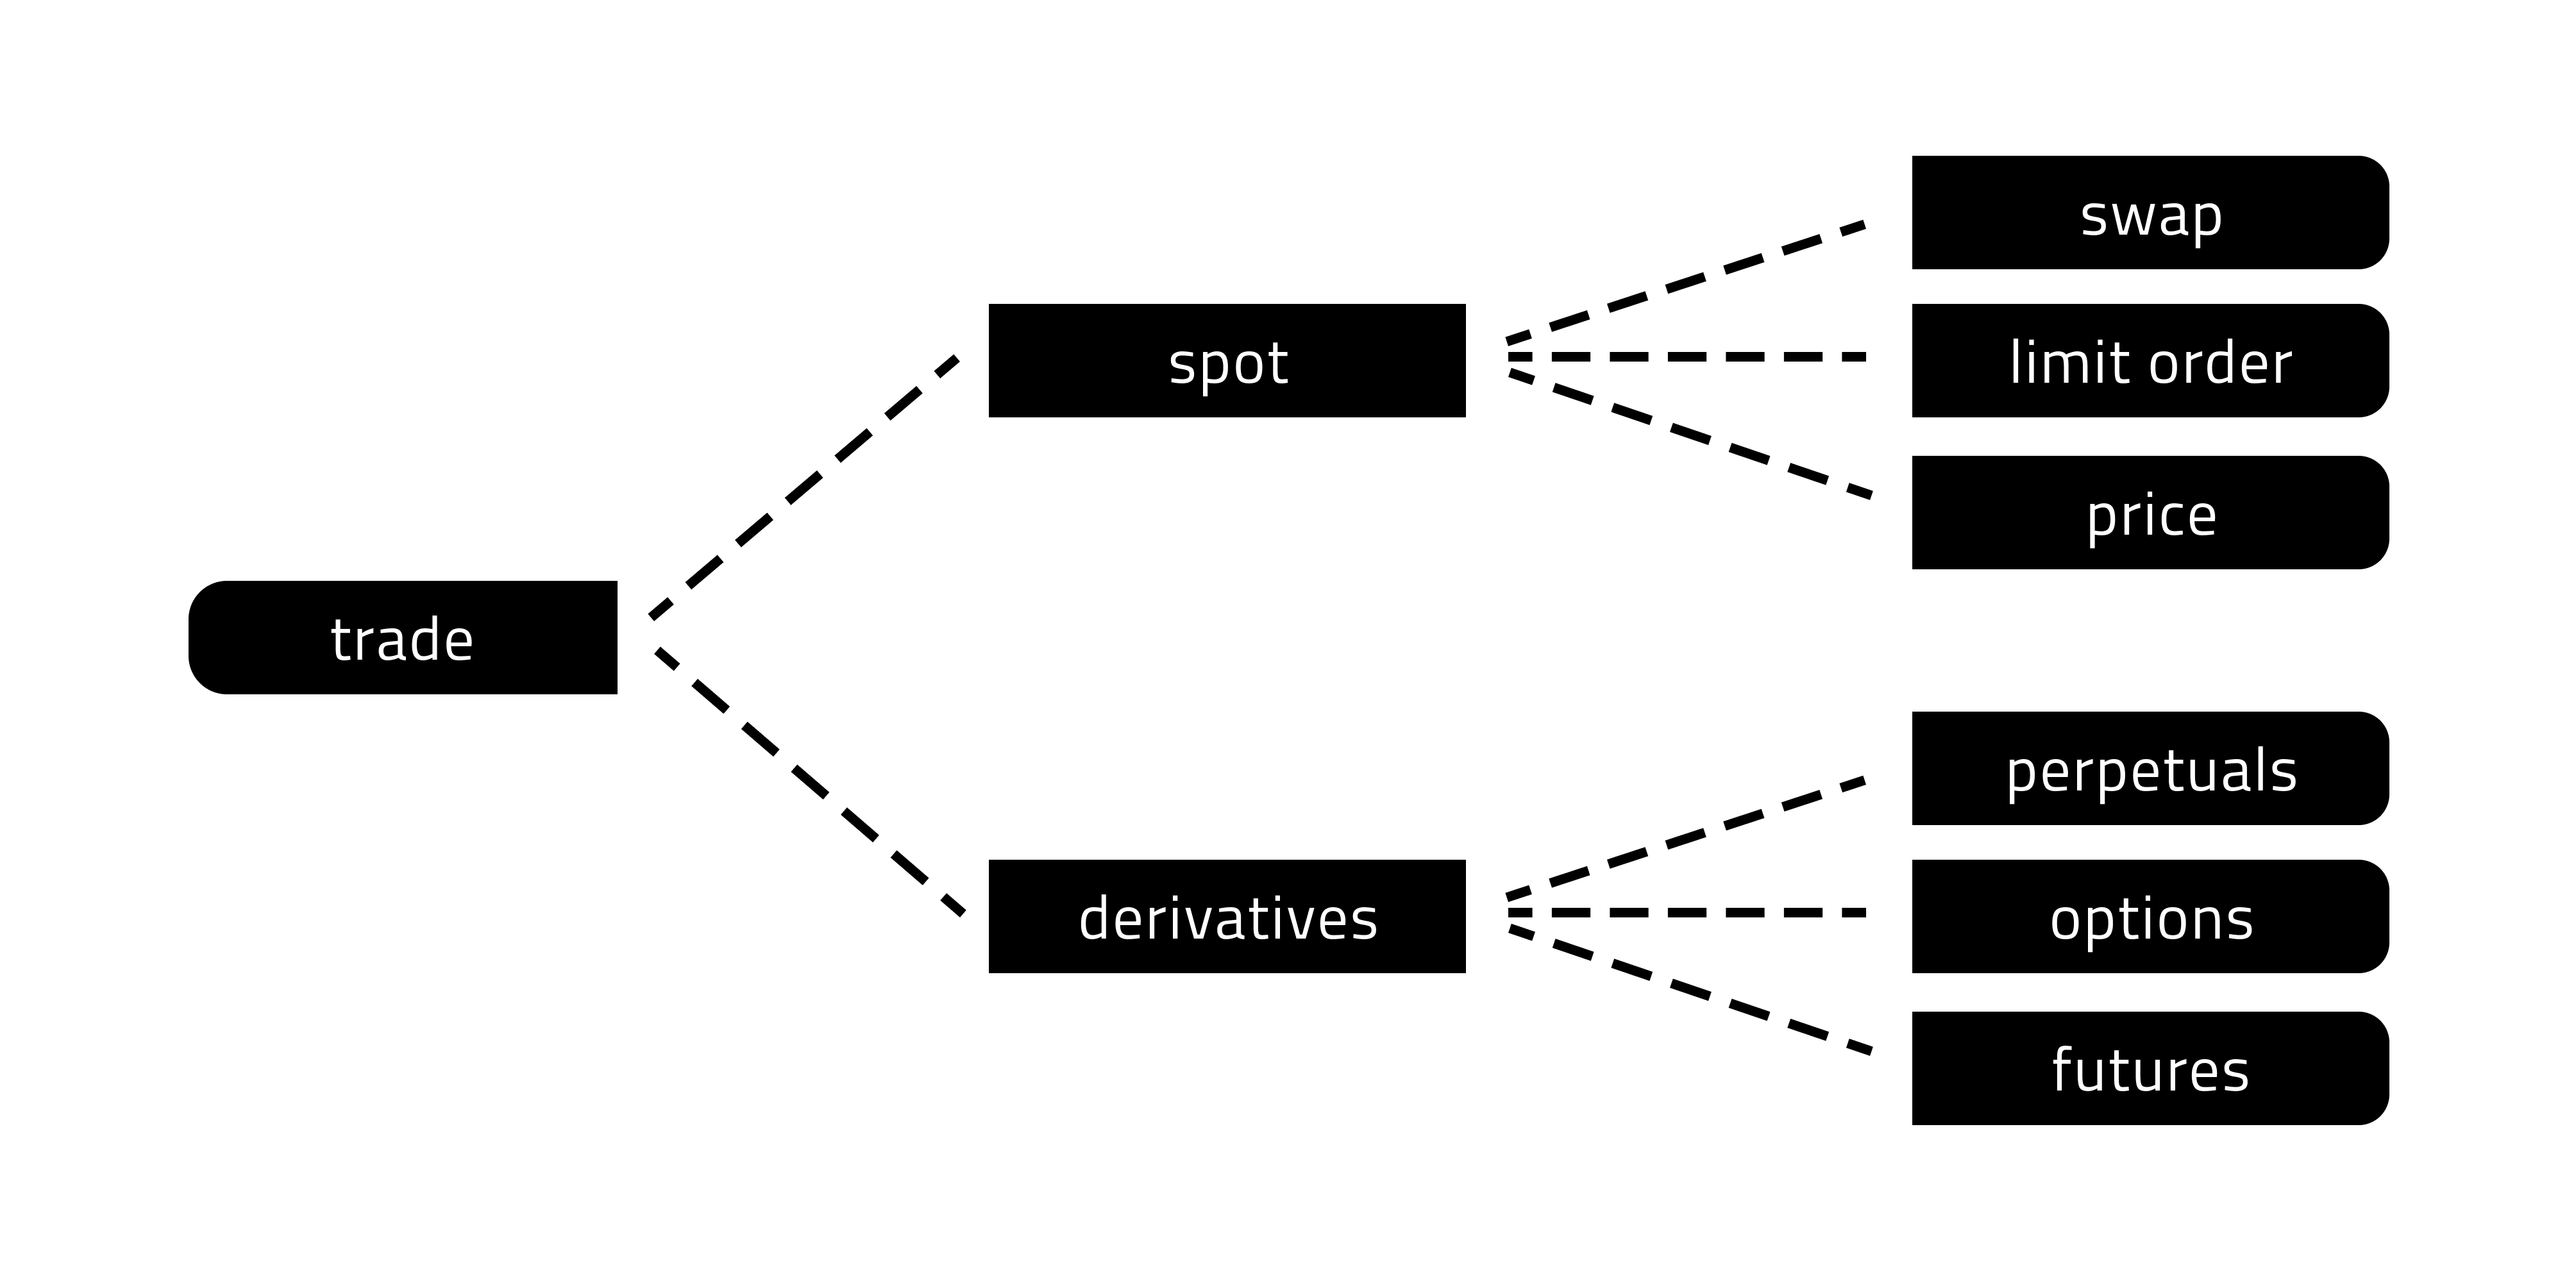
\includegraphics[width=3in]{fig/intent-taxonomy-hr.png}
\caption{An intent taxonomy is a forest of intent trees each of which represents an independent intent category.} 
\label{fig:intent-taxonomy}
\vspace{0pt}
\end{figure}

To provide unambiguous definitions, tree-based ontology is adopted. Ontology, as a branch of philosophy, is the science of what is, of the kinds and structures of objects. In simple terms, ontology seeks the classification and explanation of entities.

Nimble taxonomy is a forest formed by a set of trees. In computer science, a tree is a widely used abstract data type representing a hierarchical structure with a set of connected nodes. Each node in the tree can be connected to many children (depending on the type of tree) but must be connected to exactly one parent, except for the root node, which has no parent (i.e., the root node as the top-most node in the tree hierarchy).

Each tree defines an independent intent category. The root is the largest concept for that category. The leaf is a particular operation defined by DSL. The forest is extensible by adding new trees for new operation categories with the evolution of the Web3 concepts. Trees can be extended by adding new operations. In the example above, new derivative types can be added constantly as nodes and leaves.

The forest and leaf operations can be defined as a set of configuration files or specific code languages. The specific implementation does not matter too much, only if it is accurate. For example, operations can be defined as EVM, Move, or Rust smart contract functions, while the forest is defined as configurations. An alternative can be defined as contract programs. As a result, our definition of intent is extensible, accurate, and flexible.
\newline
\newline
\noindent \textbf{Intent Understanding.}
The outcome of intent recognizers is intent operations. Each intent operation is a leaf on a taxonomy tree. Before deep-diving intent understanding, the specification of particular intent operations is discussed. A Domain Specific Language (DSL) is a programming language with a higher level of abstraction optimized for a specific class of problems. A DSL uses the concepts and rules from the field or domain. In Web3, different intents are defined in a structured manner as a configuration or a piece of code. Below is a simple example intent \emph{swap 10 BTC for USDT at maximum $0.5\%$ slippage instantly}.

\begin{lstlisting}[style=yaml]
  intentType: swap
    from: BTC
    to: USDT
    slippageThreshold: 0.5
    amount: 10
    delay: 0
\end{lstlisting}

Despite the extensible, accurate, and flexible definitions provided by DSL, end users should not be expected to learn technical languages before using dApps. Additionally, without sophisticated knowledge of blockchain infrastructure, users may submit unsupported or irrelevant intents. Thus, developers structure intents and present them to users as familiar interactive elements like buttons, drop-down menus, etc. Once intents are submitted to the network, intent understanding aims to parse the arbitrary user inputs into specific leaf nodes in our intent taxonomy.

The intent recognizer module combines LLMs and a rules engine as illustrated in Fig. \ref{fig:intent-architecture}. There is a wide literature on this topic. Basically, rule engines define specific patterns to parse user input queries, while LLMs are a large model of neural networks used for pattern identification.
\begin{itemize}
\item \textbf{Rule Engine.} Rules engines define a set of patterns to process the intents and map intents to leaf nodes in the taxonomy forest (i.e., specific intent operations).
\item \textbf{LLM Parser.} LLMs are used for intent natural language understanding with named entity tagging by identifying salient entities, followed by specific operation classifications.
\item \textbf{DSL Mapper.} The DSL mapper combines the above parsing results for DSL formulation and intent precision boosting.
\end{itemize}

\subsection{The Dispatching Market}
The Intent Dispatching Layer is a crucial intermediary between the intent recognizers and solvers. It plays a multifaceted role in optimizing and safeguarding user operations as they move through the protocol.

Its primary responsibility is efficiently managing and organizing these operations as they flow in from the Intent Recognition Layer. Using event-driven architecture and real-time data batching, this layer ensures that user operations are processed in an orderly fashion. It employs a bundling mechanism to group-related operations, reducing blockchain network congestion and optimizing gas costs. By sequencing and prioritizing intent operations, it maintains the consistency and integrity of the blockchain network. This layer acts as the traffic controller and matching protocol, directing intent operations toward solvers for validation and execution, ensuring a streamlined and efficient process.

Additionally, this layer verifies the authenticity and integrity of each operation by checking the associated digital signatures, which must be validated to ensure that the operations originate from authorized users and have not been tampered with during transit. Furthermore, this layer implements business logic rules and access control policies. It enforces constraints and conditions on user operations to prevent unauthorized or malicious actions, ensuring that only valid and secure operations proceed to the solvers.

\begin{itemize}
    \item Positioned as the middleware layer between intent recognition and execution, the intent dispatching layer optimizes and organizes intent operations.

    \item Consists of bundling operations with specialized optimization algorithms.
    
    \item Optimizes and bundles related intent operations for more efficient execution to reduce blockchain network congestion and optimize gas costs.

    \item Ensures proper sequencing and prioritization of operations to maintain consistency and integrity in the blockchain network.
\end{itemize}
\newline
\newline
\noindent \textbf{Privacy Considerations.} Dispatching involves two processes:
revealing intents to solvers and revealing auction bids
to the network. For the initial launch, solvers participate
in the network with staking. Intents are batched for
processing to minimize cheating behaviors. In later network releases, fully homomorphic encryption (FHE) will be implemented to enable private computations on encrypted data \cite{fhe2023zama}.

\subsection{The Settlement Market}
The Intent Execution Layer serves as the engine that transforms user intentions into tangible blockchain actions, and it introduces an innovative element known as the Solver Network to provide extensibility. Within this layer, the protocol’s primary function is to leverage the Solver Network - a decentralized group of nodes specializing in different dApp and blockchain operations - to solve user’s intents while introducing competition at every stage.

These specialized nodes form a decentralized marketplace of computational resources, offering their expertise and computational power to compete and find optimal solutions for user intents. For instance, some nodes might specialize in decentralized finance (DeFi) operations, while others focus on non-fungible tokens (NFTs), smart contract interactions, or decentralized storage solutions.

The Solver Network ensures that users receive efficient, cost-effective, and timely results for their intents, harnessing the collective intelligence of a decentralized community of experts. This layer coordinates and manages the interactions with the Solver Network, ensuring fair competition, transparent decision-making, and efficient resource allocation. The protocol -

\begin{itemize}
    \item Cooperates with a solver network that leverages optimization algorithms, smart contract scripting, and decentralized finance (DeFi) protocols to competitively find the best solution to execute user operations.

    \item Ensures anyone can join the solver network, deploy their own algorithms, and compete for the best solution to satisfy user intents.
    \item Generates modular auctions for each operation supported by each solver. Multi-function auctions are generated for common user actions, allowing optimal solutions to be discovered where intents span more than one operation.
\end{itemize}


\subsection{Multi-chain Contracts}
\label{sec:intent-peripherals}
User intent classes, execution, dispatching, validation, and error handling are key components of the intent contract. We focus our discussions on the intent class, execution, and dispatching since validation and error handling come naturally. The UserIntents class defines intents through the taxonomy. It also consists of important intent utility functions. The IntentDispatcher is the unified interface for solvers to interact with, and it routes intents to specialized IntentExecutor. IntentExecutor class handles particular intent operation executions. Intents are validated before being sent to the IntentDispatcher. ErrorHandler is called by different components whenever errors are detected. The flow is illustrated in
Fig. \ref{fig:intent-architecture}.

\section{Modular Mechanism Design}
\label{sec:mechanism}

\begin{figure}[t]
\centering
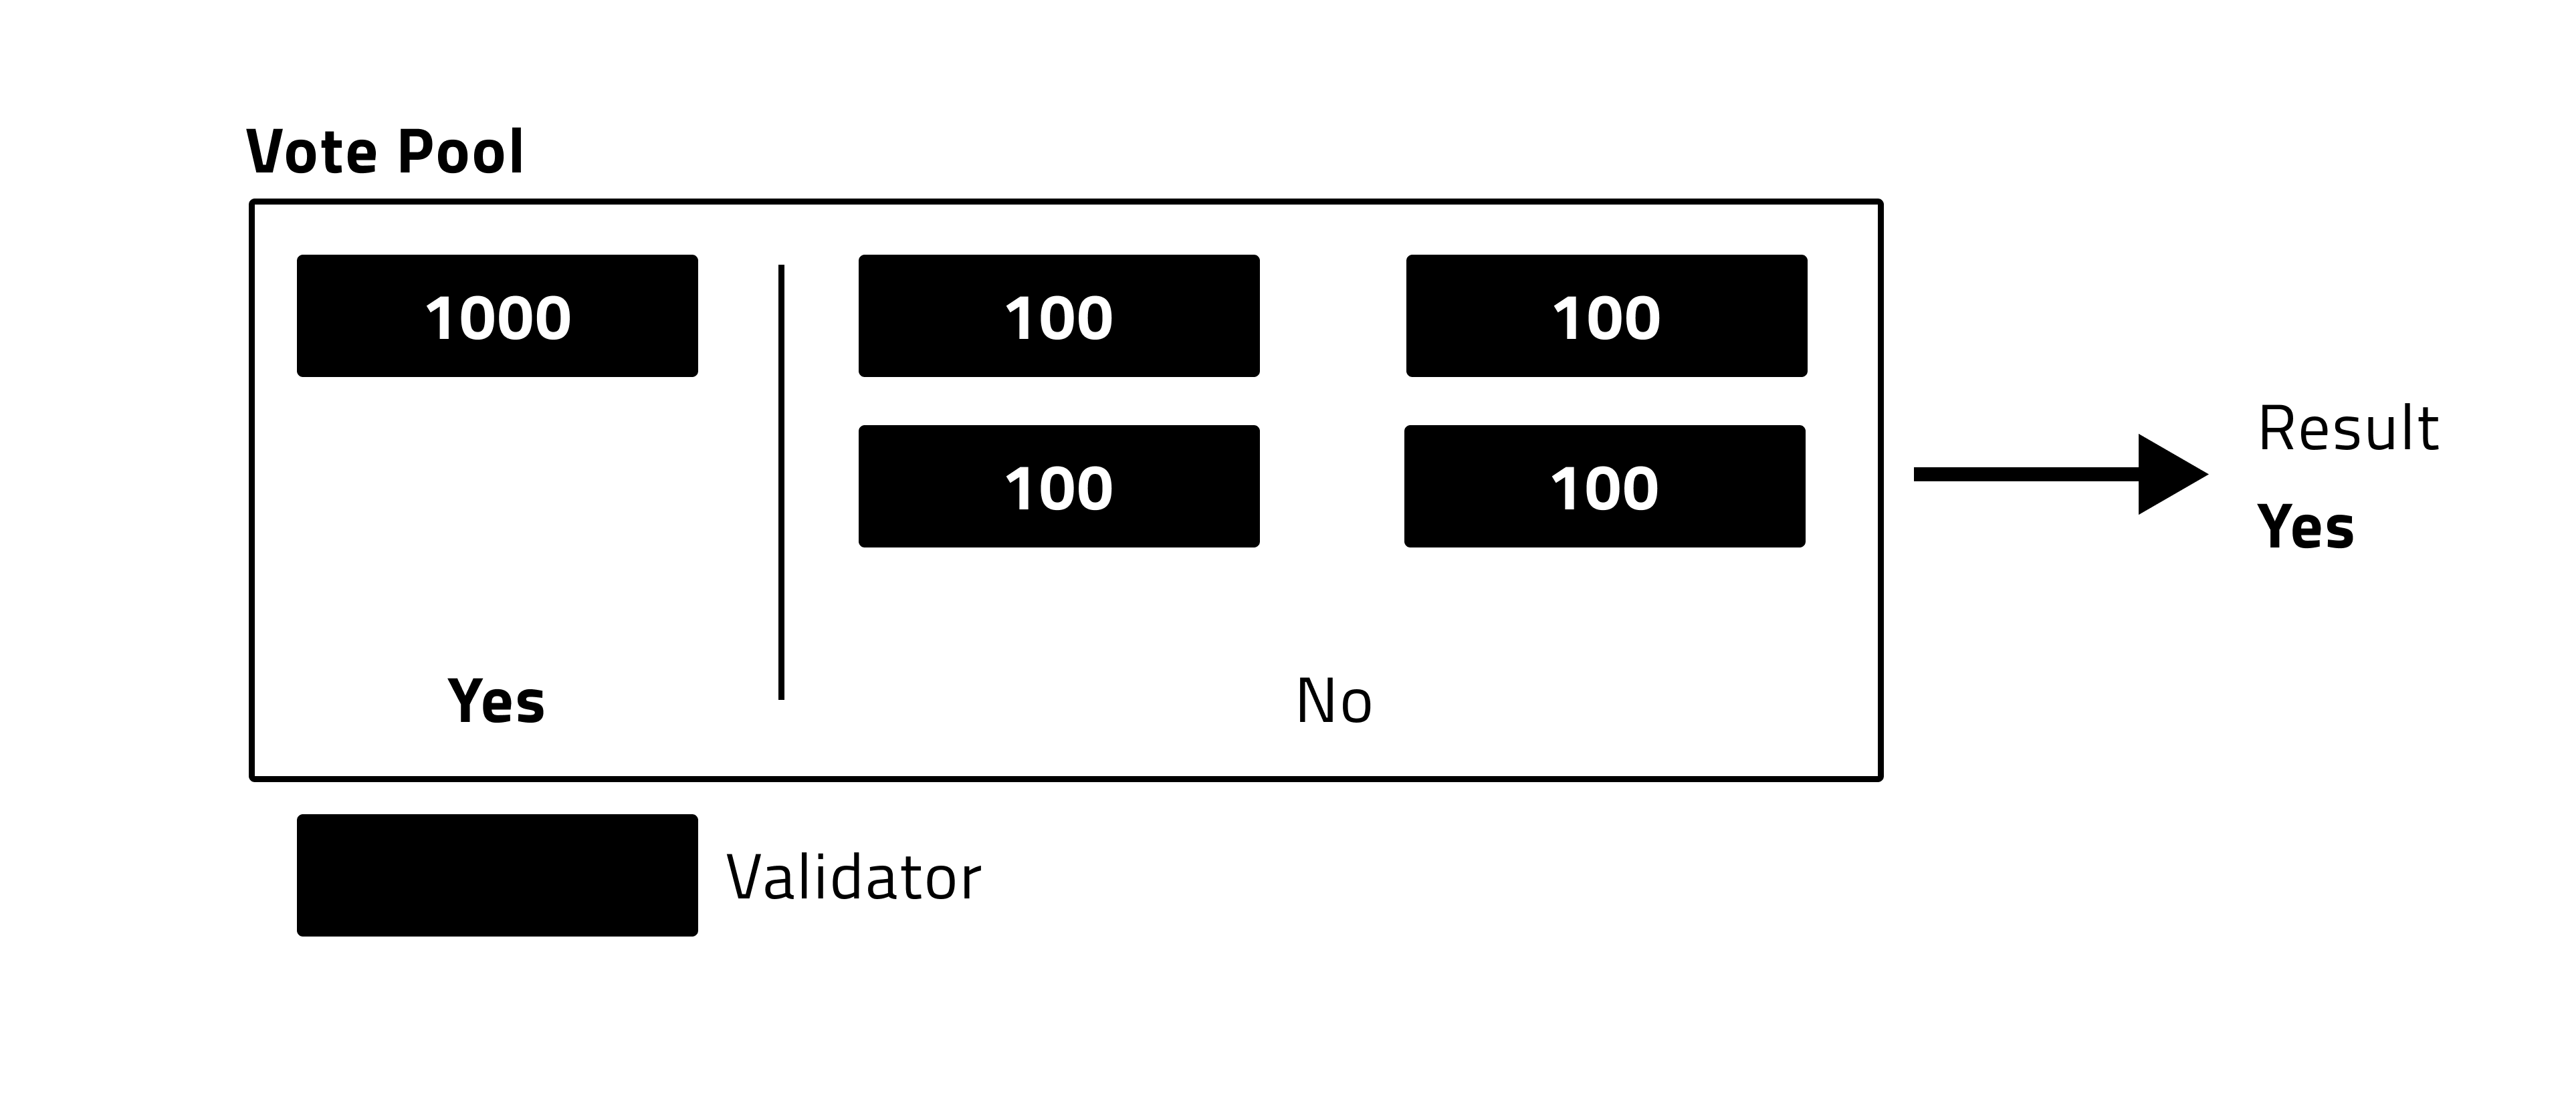
\includegraphics[width=3in]{fig/weighted-voting-hr.png}
\caption{A simple example of weighted voting for model predictions with binary classifications.} 
\label{fig:weighted-voting}
\vspace{0pt}
\end{figure}

As discussed in Section \ref{sec:introduction}, the intent mechanism design consists of the mediator (i.e., the network governed by
the Nimble consensus) and the solvers, all of which are autonomous agents optimizing for their self-interest. Generic
solvers may fulfill the entirety of a user’s
intent, while specialized solvers may fulfill only a single operation in a highly optimized way.

For generality, the rest of this section's discussions focus on specialized solvers.

Two categories of solvers participate in the Nimble protocol. Processors are defined as
solvers that operate on sub-operations of users' intents. Processors perform operations like swap, transfer, and so on.
Processors unpack intents into multiple transactions and then submit a separate intent for bundling.
Bundlers are defined as solvers that handle block-building
intents.

In such a multi-agent setting with mediators, processors, and bundlers, an \emph{outcome} is an allocation of intents among
processors. Each allocation is sequenced and executed on-chain by
bundlers. This becomes a multi-stage mechanism design problem
\cite{myerson1986multistage, jurca2009mechanisms, curry2023automated, sandholm2007automated, hajiaghayi2007automated, gan2022sequential}. In our modular design, the multi-stage game is modeled as independent second-price sealed-bid auctions (i.e., a special
case of Vickrey auctions) for agent bid truthfulness
\cite{laffont1980optimal, ausubel1999generalized}.

\section{Nimble Consensus}
\label{sec:consensus}

\begin{figure}[t]
\centering
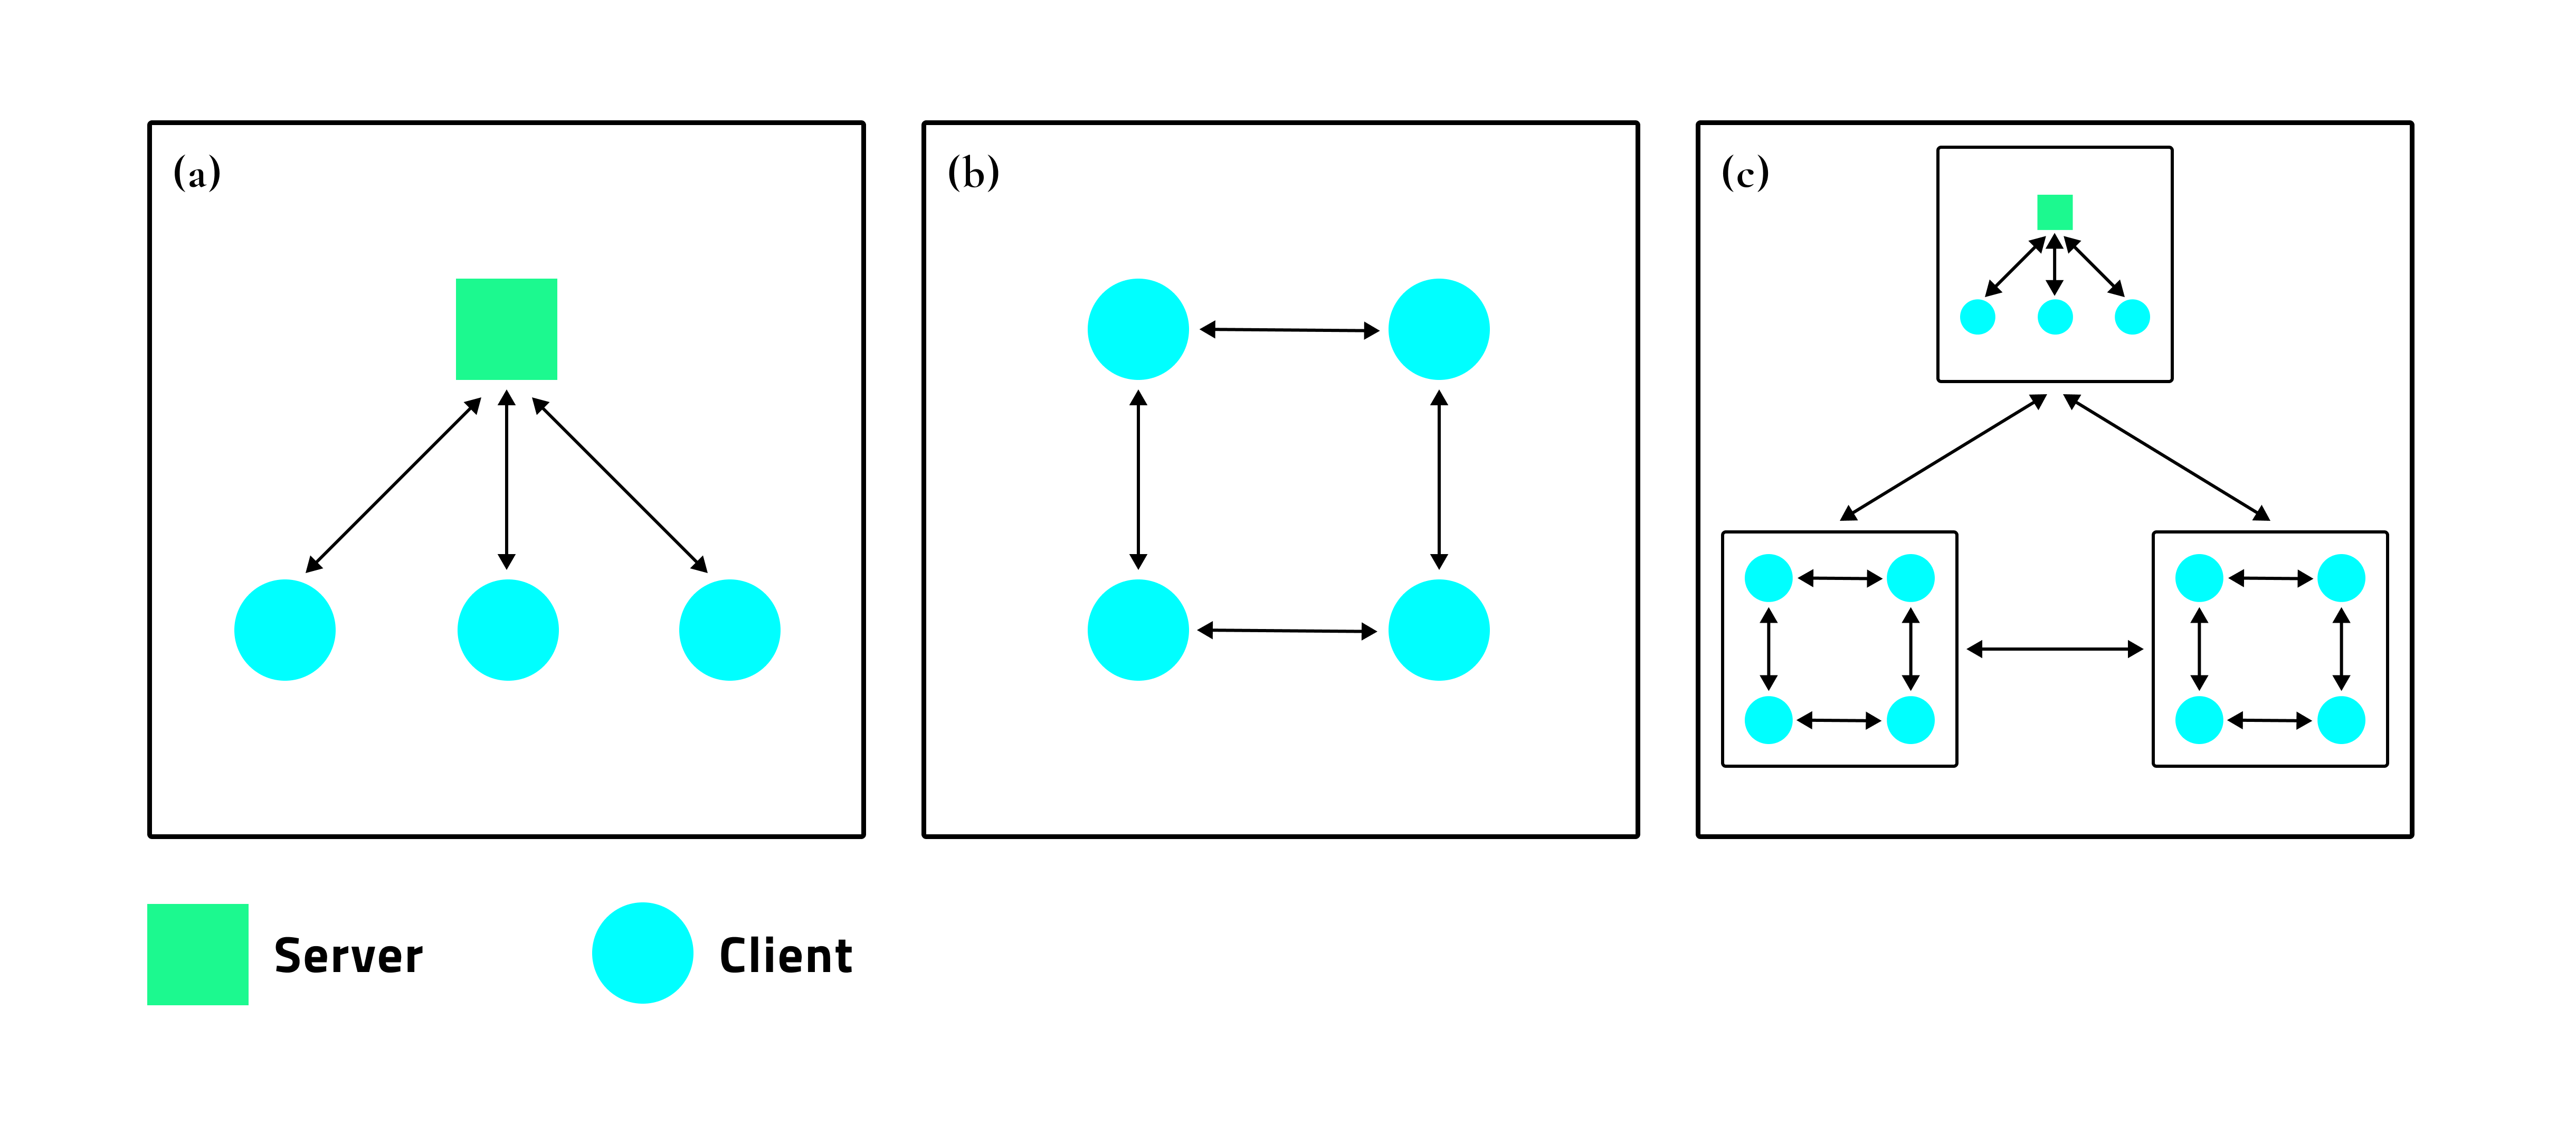
\includegraphics[width=3in]{fig/decentralized-learning-hr.png}
\caption{A comparison of centralized and decentralized learning. a) centralized learning, b) decentralized learning, and c) decentralized
learning with each validator running one or more network nodes.} 
\label{fig:decentralized-learning}
\vspace{0pt}
\end{figure}

\begin{figure}[b]
\centering
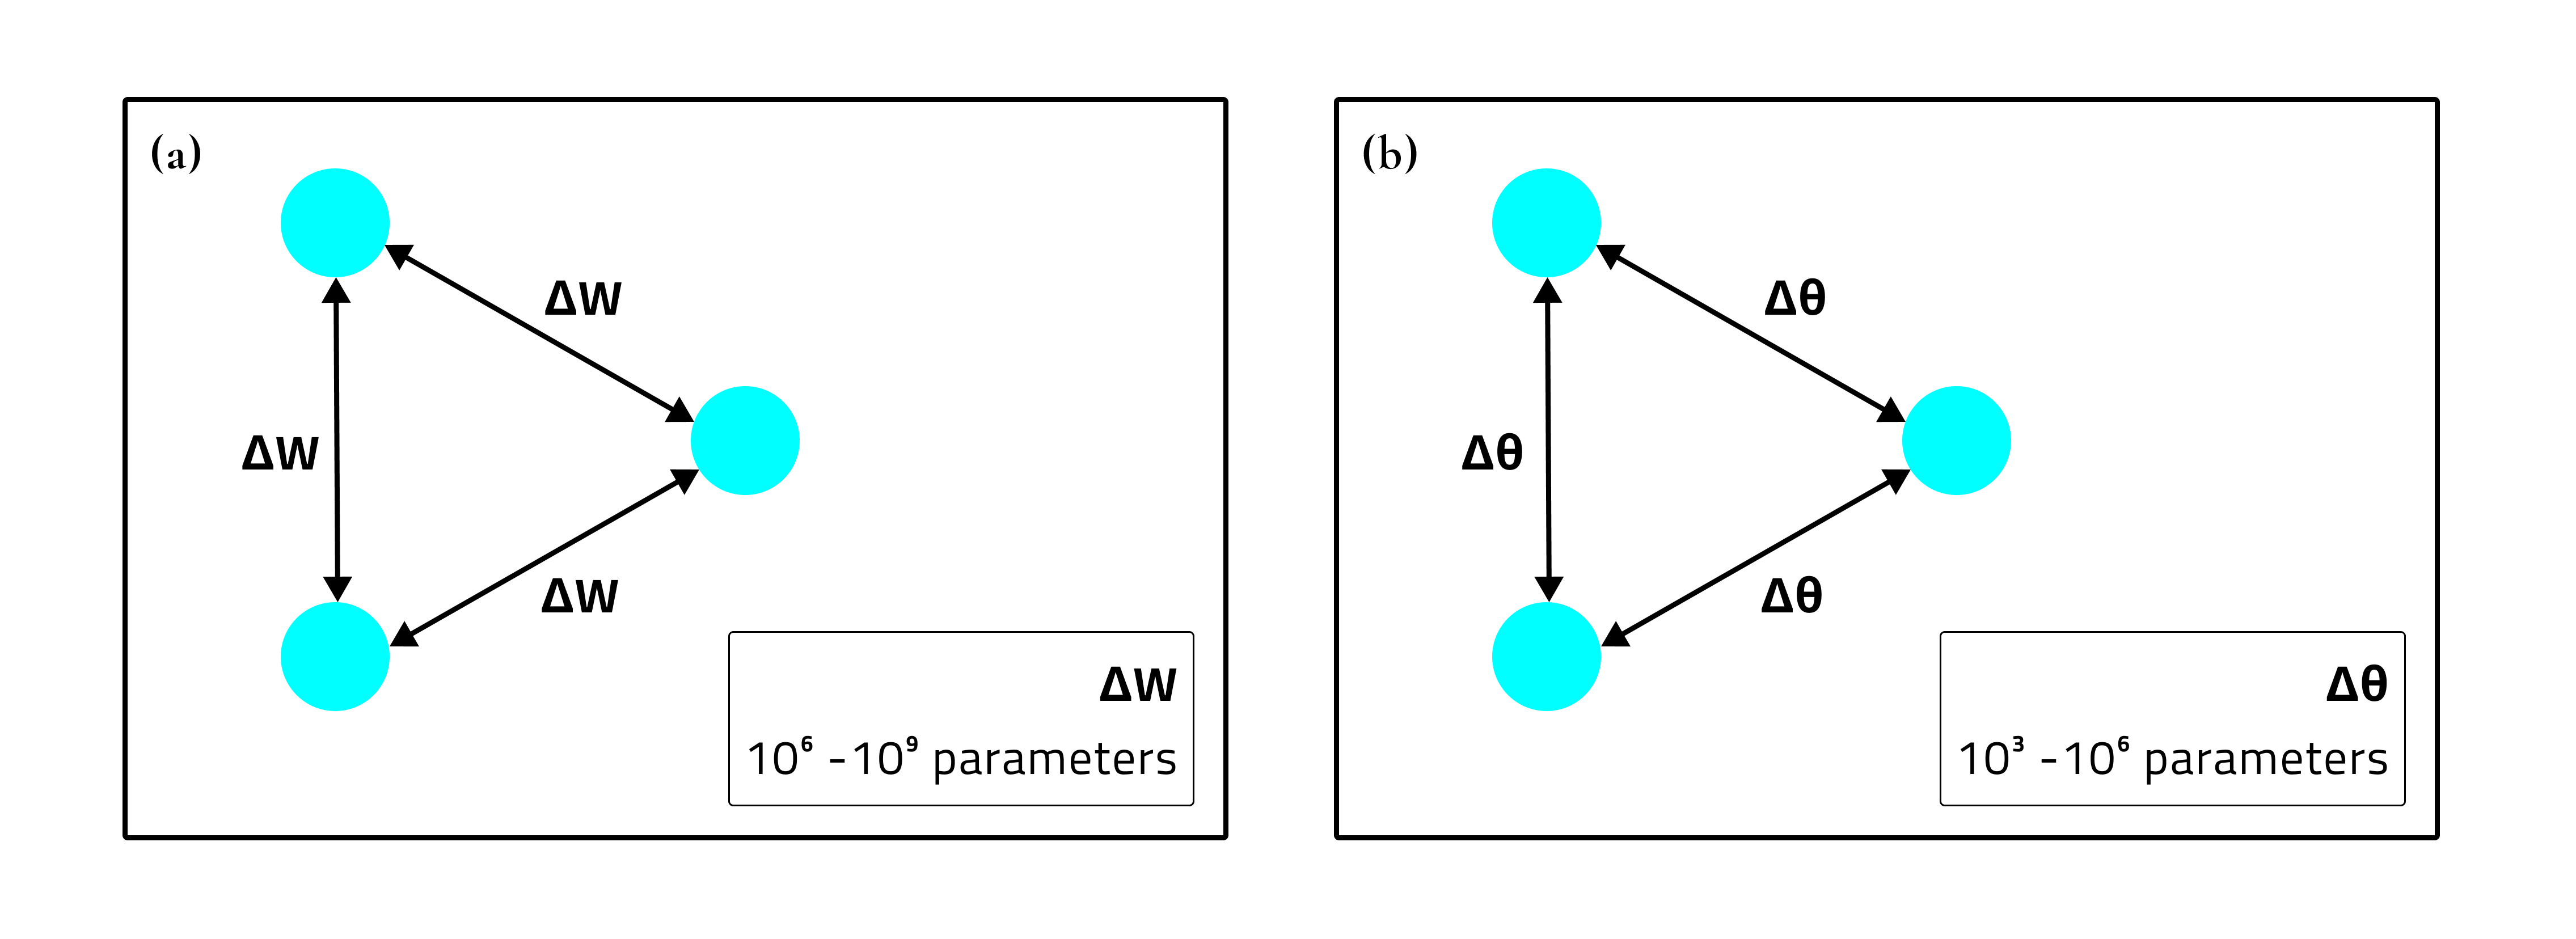
\includegraphics[width=3in]{fig/compressed-learning-hr.png}
\caption{With compressed learning, model parameters can be compressed up to $1,000$ times without sacrificing model performances.} 
\label{fig:compressed-learning}
\vspace{0pt}
\end{figure}

To participate in network consensus validation, validators must 
have a minimum amount of staked Nimble tokens. The staked amounts proportionately affect the $2f + 1$ stake
weighted \emph{PoAv} during intent dissemination, vote weights, and leader selection during intent recognition and ordering. Validators decide on the split of rewards between themselves and their
respective stakers. Stakers can select any number of validators to stake their tokens for a
pre-agreed reward split. At the end of every epoch, validators and their respective stakers will receive
their rewards via the relevant on-chain modules.
Any validator operator with sufficient stake can freely join the Nimble consensus. The network enablement processes can set all parameters,
including the minimum stake required.
\newline
\newline
\noindent \textbf{Intent Mining.} Intents coming from users and dApps need to be processed by the network for model updates (e.g., intent understanding model, AI routing, and general purpose intent understanding). Validators are rewarded by improving model performances with new intent data and serving intent requests. Users earn network
tokens by contributing data. DApps pay network fees for intent requests. Early users get more network tokens due to diminishing network token emission rates.
\newline
\newline
\noindent \textbf{Interpretation Market.} Let us use the interpretation market consensus as a case study. Network validators own one single interpretation model, as standardized by intent DSL. It of
different model stages such as spelling corrections, query
segmentation, query expansion, named entity tagging and structured intent DSL mapping.
At the inference stage, validators apply
weighted voting as illustrated in Fig. \ref{fig:weighted-voting} for the binary classification example. For the initial launch, the network only decentralizes inferences and updates
models with a voting governance mechanism by evaluating the model performance against a predefined validation intent set. In the future, the training can also be decentralized with
decentralized learning \cite{lalitha2018fully, li2020federated, sattler2019robust} as illustrated in Fig. \ref{fig:decentralized-learning}
and the model parameters are compressed for efficient network
transmission  \cite{yang2022hardware, chen2022self, zhang2021fpga, hawkins2021bayesian, hawkins2022towards, roh2021sample} (e.g., as illustrated in Fig. \ref{fig:compressed-learning}).

\section{Conclusion}
\label{sec:conclusion}
In conclusion, the \emph{Nimble marketplace infrastructure} we are diligently crafting represents a pivotal leap forward in the realm of Web3 and blockchain technology. This innovative framework bridges the communication chasm between users and decentralized networks, offering a seamless and intuitive means to articulate complex intentions within this intricate digital landscape. By encapsulating the essence of human intent within a structured query language, we empower individuals to navigate the Web3 ecosystem with unparalleled ease and precision.


Our primary objective is to significantly lower the bar for users to enter the Web3 world. Our intent protocol paves the way for a harmonious collaboration between human cognition and the decentralized world through natural language processing, LLMs, and blockchain expertise. It promises a future where blockchain interactions are as effortless as conversing in plain language, all while upholding the security and integrity of blockchain transactions.


With our intent marketplace solution, we venture into uncharted territory, shaping the future of Web3 by democratizing access to the blockchain. This groundbreaking initiative is a testament to our commitment to enhancing user experiences, catalyzing innovation, and ultimately transforming how we interact with the digital frontier. As we continue to refine and expand upon this vision, we invite you to join us on this remarkable journey into the future of Web3. Together, we shall redefine the possibilities of human-machine collaboration in the blockchain era, making the Web3 world more accessible and inclusive than ever before.

\bibliography{Bibliography}
\bibliographystyle{plain}

\end{document}
